% This is based on "sig-alternate.tex" V1.9 April 2009
% This file should be compiled with V2.4 of "sig-alternate.cls" April 2009
%
\documentclass{report}

\usepackage[english,german]{babel}
\usepackage[utf8x]{inputenc}
\usepackage{graphicx}
\usepackage{tabularx}
\usepackage{subfigure}
\usepackage{enumitem}
\usepackage{url}
\usepackage{float}

\usepackage{color}
\definecolor{orange}{rgb}{1,0.5,0}
\definecolor{lightgray}{rgb}{.9,.9,.9}
\definecolor{java_keyword}{rgb}{0.37, 0.08, 0.25}
\definecolor{java_string}{rgb}{0.06, 0.10, 0.98}
\definecolor{java_comment}{rgb}{0.12, 0.38, 0.18}
\definecolor{java_doc}{rgb}{0.25,0.35,0.75}

% code listings

\usepackage{listings}
\lstloadlanguages{Java}
\lstset{
	language=Java,
	basicstyle=\scriptsize\ttfamily,
	backgroundcolor=\color{lightgray},
	keywordstyle=\color{java_keyword}\bfseries,
	stringstyle=\color{java_string},
	commentstyle=\color{java_comment},
	morecomment=[s][\color{java_doc}]{/**}{*/},
	tabsize=2,
	showtabs=false,
	extendedchars=true,
	showstringspaces=false,
	showspaces=false,
	breaklines=true,
	numbers=left,
	numberstyle=\tiny,
	numbersep=6pt,
	xleftmargin=3pt,
	xrightmargin=3pt,
	framexleftmargin=3pt,
	framexrightmargin=3pt,
	captionpos=b
}

% Disable single lines at the start of a paragraph (Schusterjungen)

\clubpenalty = 10000

% Disable single lines at the end of a paragraph (Hurenkinder)

\widowpenalty = 10000
\displaywidowpenalty = 10000
 
% allows for colored, easy-to-find todos

\newcommand{\todo}[1]{\textsf{\textbf{\textcolor{orange}{[[#1]]}}}}

% consistent references: use these instead of \label and \ref

\newcommand{\lsec}[1]{\label{sec:#1}}
\newcommand{\lssec}[1]{\label{ssec:#1}}
\newcommand{\lfig}[1]{\label{fig:#1}}
\newcommand{\ltab}[1]{\label{tab:#1}}
\newcommand{\rsec}[1]{Section~\ref{sec:#1}}
\newcommand{\rssec}[1]{Section~\ref{ssec:#1}}
\newcommand{\rfig}[1]{Figure~\ref{fig:#1}}
\newcommand{\rtab}[1]{Table~\ref{tab:#1}}
\newcommand{\rlst}[1]{Listing~\ref{#1}}

% General information

\title{Distributed Systems -- Assignment 4 - Report}

% Use the \alignauthor commands to handle the names
% and affiliations for an 'aesthetic maximum' of six authors.

\numberofauthors{3} %  in this sample file, there are a *total*
% of EIGHT authors. SIX appear on the 'first-page' (for formatting
% reasons) and the remaining two appear in the \additionalauthors section.
%
\author{
% You can go ahead and credit any number of authors here,
% e.g. one 'row of three' or two rows (consisting of one row of three
% and a second row of one, two or three).
%
% The command \alignauthor (no curly braces needed) should
% precede each author name, affiliation/snail-mail address and
% e-mail address. Additionally, tag each line of
% affiliation/address with \affaddr, and tag the
% e-mail address with \email.
%
% 1st. author
\alignauthor Lukas Gianinazzi\\
	\affaddr{ETH ID 11-719-143}\\
	\email{glukas@student.ethz.ch}
% 2nd. author
\alignauthor Mathias Birrer\\
	\affaddr{ETH ID 11-921-129}\\
	\email{matbirre@student.ethz.ch}
% 3rd. author
\alignauthor Vincent Demotz\\
	\affaddr{ETH ID 12-929-188}\\
	\email{vdemotz@student.ethz.ch}
\and  % use '\and' if you need 'another row' of author names
% 4th. author
\alignauthor Young Ban\\
 	\affaddr{ETH ID 10-935-062}\\
 	\email{bany@student.ethz.ch}
% 5th. author
\alignauthor Alessio Bähler\\
 	\affaddr{ETH ID XX-XXX-XXX}\\
 	\email{abaehler@student.ethz.ch}
% 6th. author
\alignauthor Samuel Schmid\\
 	\affaddr{ETH ID 10-919-991}\\
 	\email{schmisam@student.ethz.ch}
}


\begin{document}

\maketitle

\begin{abstract}
Social is an Android application that allows users to share thoughts and impressions with their friends by posting text or image messages on their profiles.
The distinctive feature of Social is that instead of using a client-server architecture like todays well known social networks, which store all data on a server, it uses a peer-to-peer approach and only stores data on user devices, giving them a better control over their own data.
The motivation to provide a social networking service that focuses on privacy and security comes from the invasive privacy policies that such communication services nowadays have.
\end{abstract}

\section{Problem Statement}

Going into this project we considered following problems we would have to solve: \newline
Consistent storage/retrieval of posts and information:  \newline
We have to make sure that if an user posts on a wall every user able to access that wall should get it immediately if online or be able to retrieve it later. This ensures that eventually every user sees the same posts.  \newline
Logical consistency of the posts:  \newline
Posts user make with the knowledge of certain post should be displayed after that post.  \newline
Encryption of the posts and information in a suitable way:  \newline
Posting on a certain wall should only require to encrypt the post once. Every friend of the owner of the wall should be able to read the post but noone else. \newline

%\vspace{-20mm} % use negative white space to fix too large gaps

\section{Architecture}

The system consists of a set of peers. Those peers use a server to relay messages to each other. The server keeps a cache of recent posts. If a peer is not available the server can serve posts from that cache. If a peer posts to an offline peer, the server buffers that message until the recipient gets back online. When online, peers receive 
updates to their own walls by a "push" mechanism.

\section{Implementation}

The implementation consist of the following components: On the client side, there is the User Interface, Database, Security, and Protocol implementation. The server is very lightweight and consists of a single component.

\subsection{User Interface}

The main activity holds a navigation bar to switch between the friends list and the user's own wall (a).

A second activity is for viewing a friend's wall. This activity is started when clicking one of the friends (b) or immediately after establishing a new friendship. The wall is implmented using the same fragment the user sees when looking at his or her own wall.\newline

The last activity is for displaying incoming friendship requests. It pops up when two phones are held close together and one of the users taps the screen, initiating a friendship request (c).


\begin{figure}[H]
	\centering
	\subfigure[]{
		
	    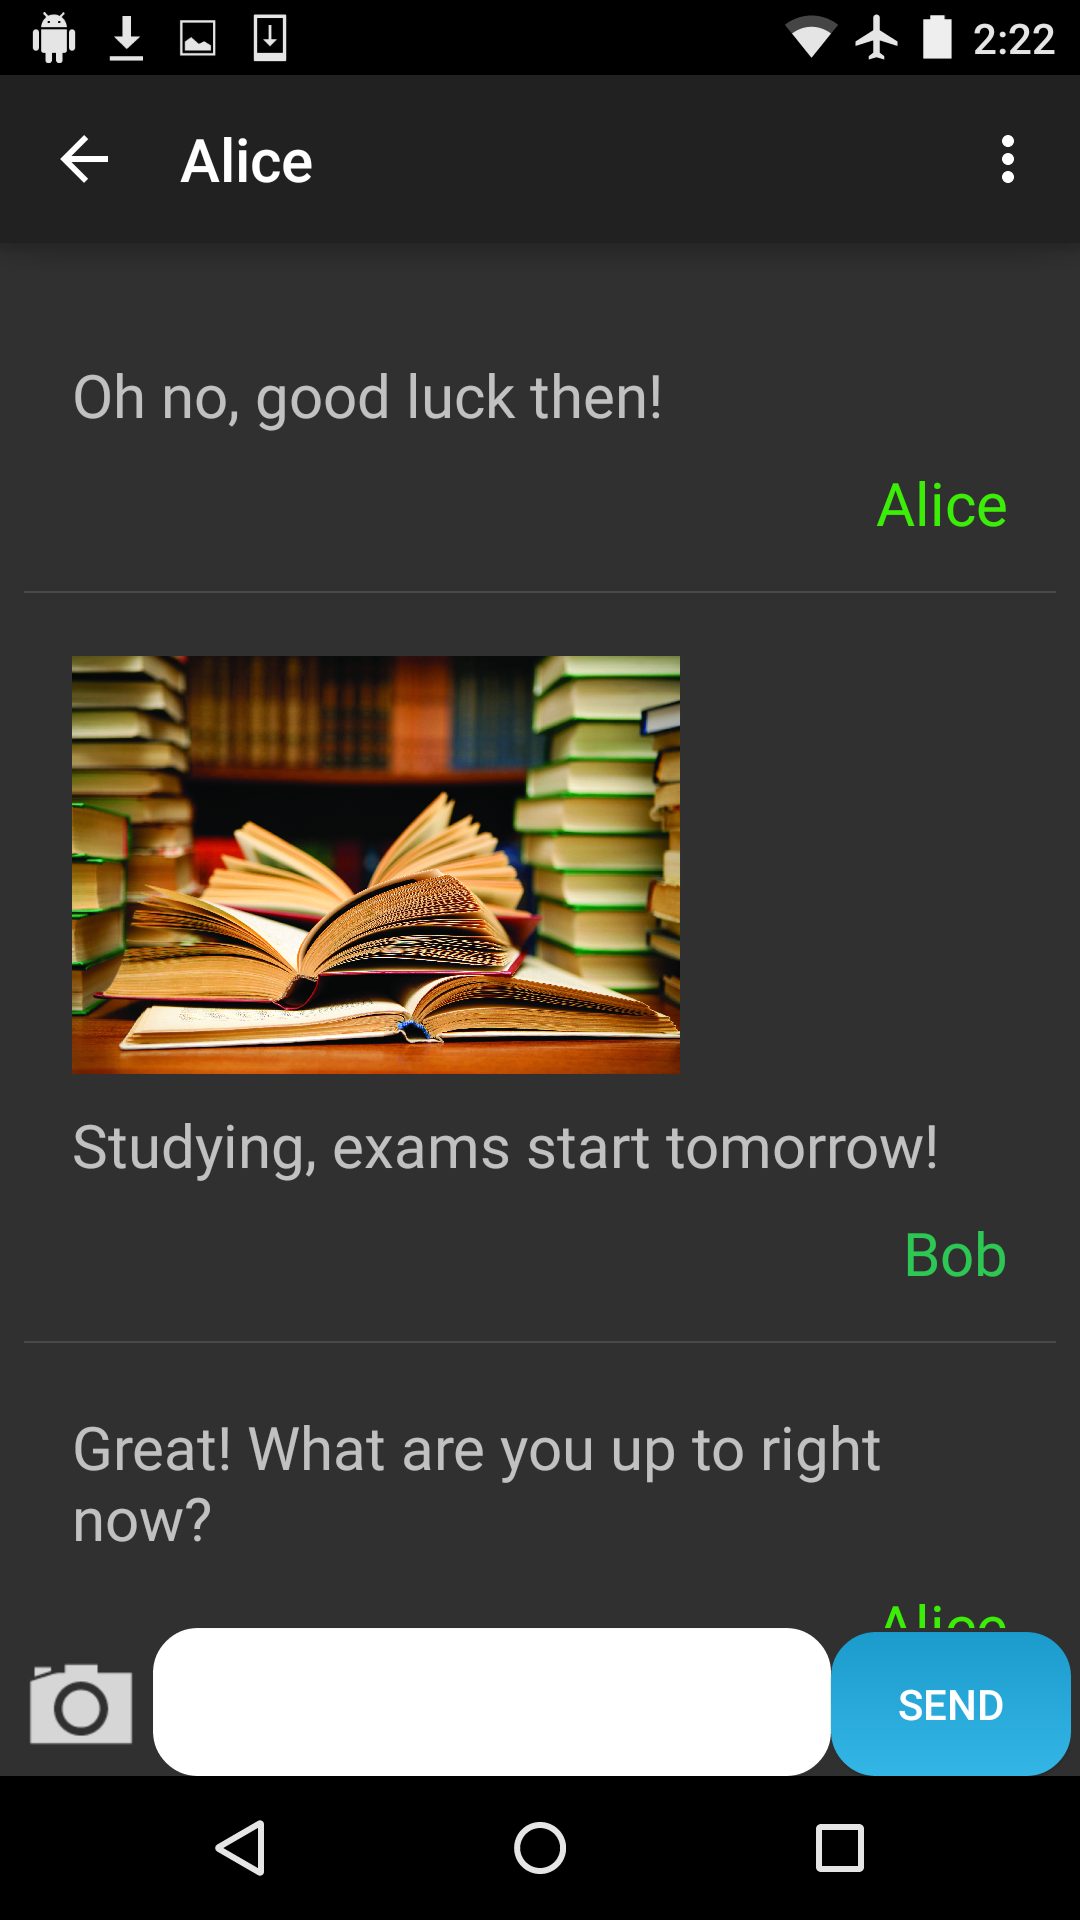
\includegraphics[height=4.5cm]{Figure_1}
	}
	\hfill
	\subfigure[]{
	    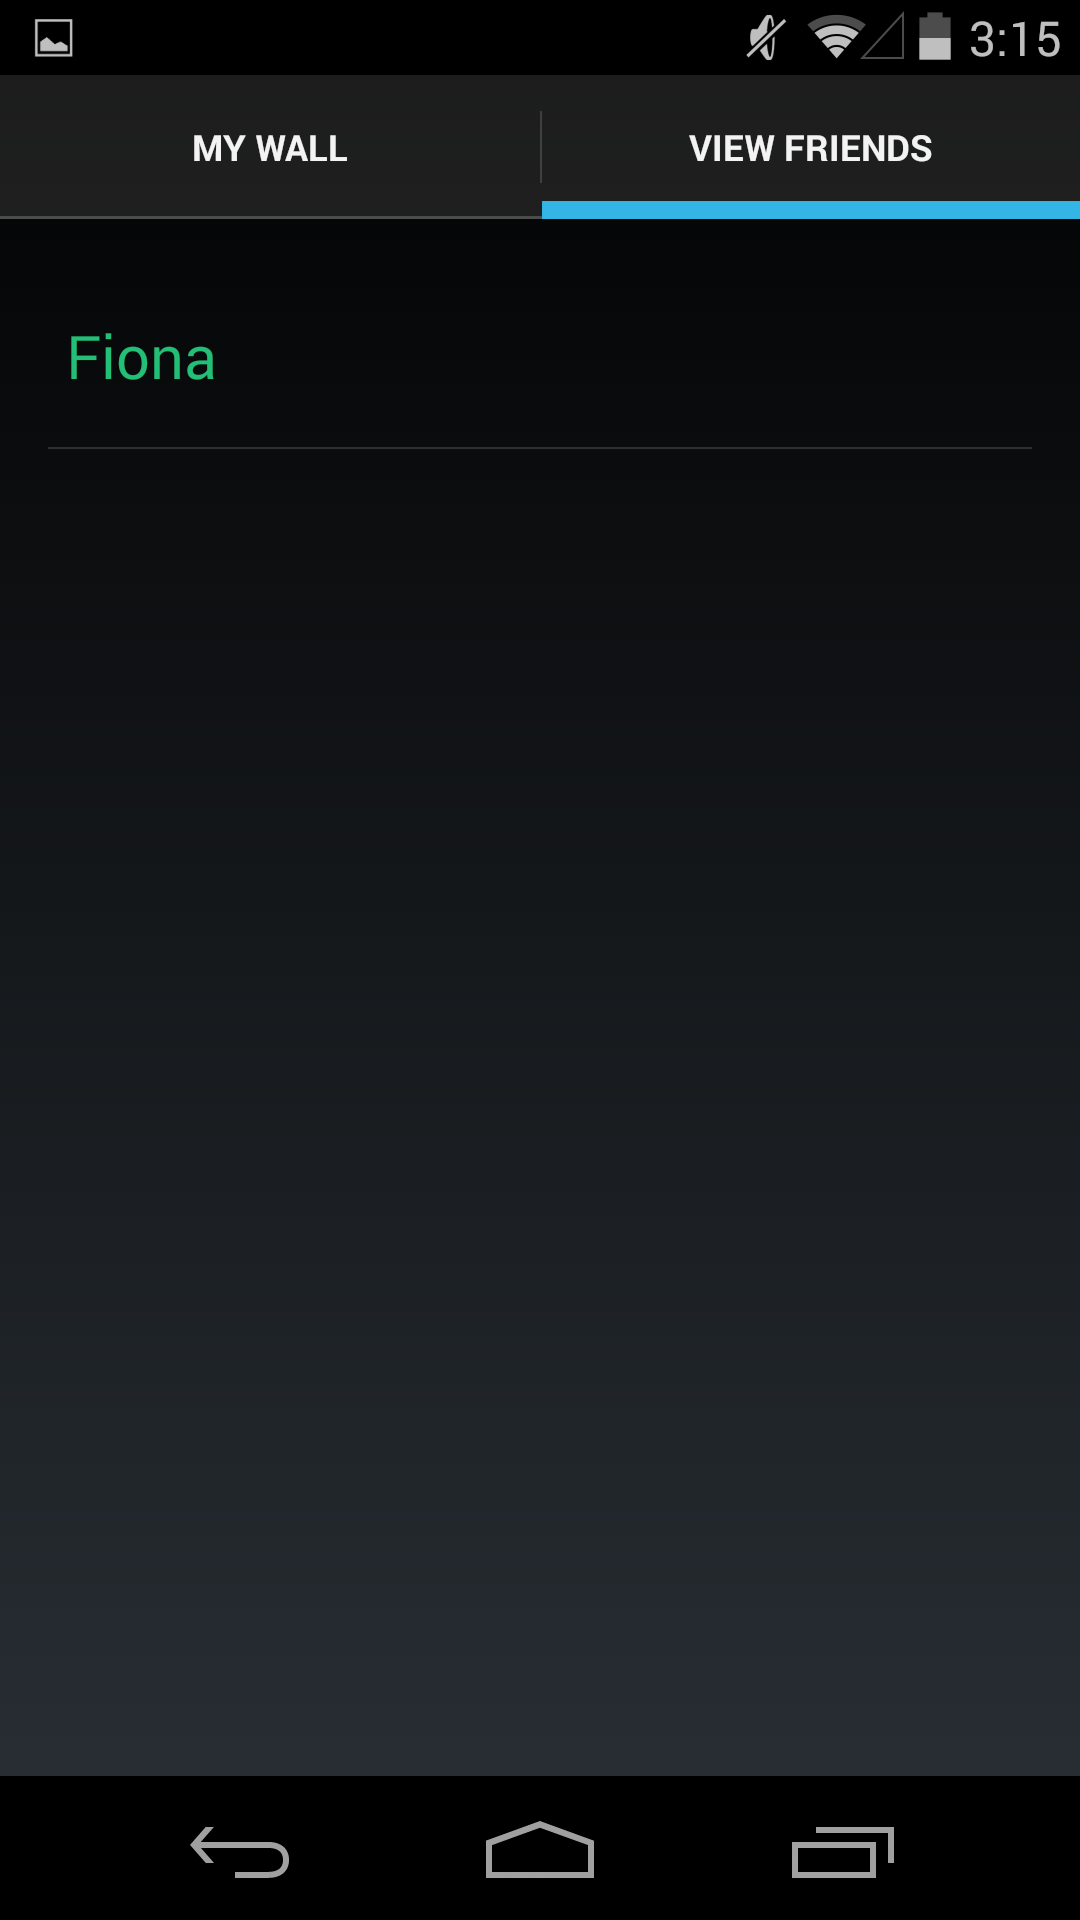
\includegraphics[height=4.5cm]{Figure_2}

	}
	\hfill
	\subfigure[]{
	    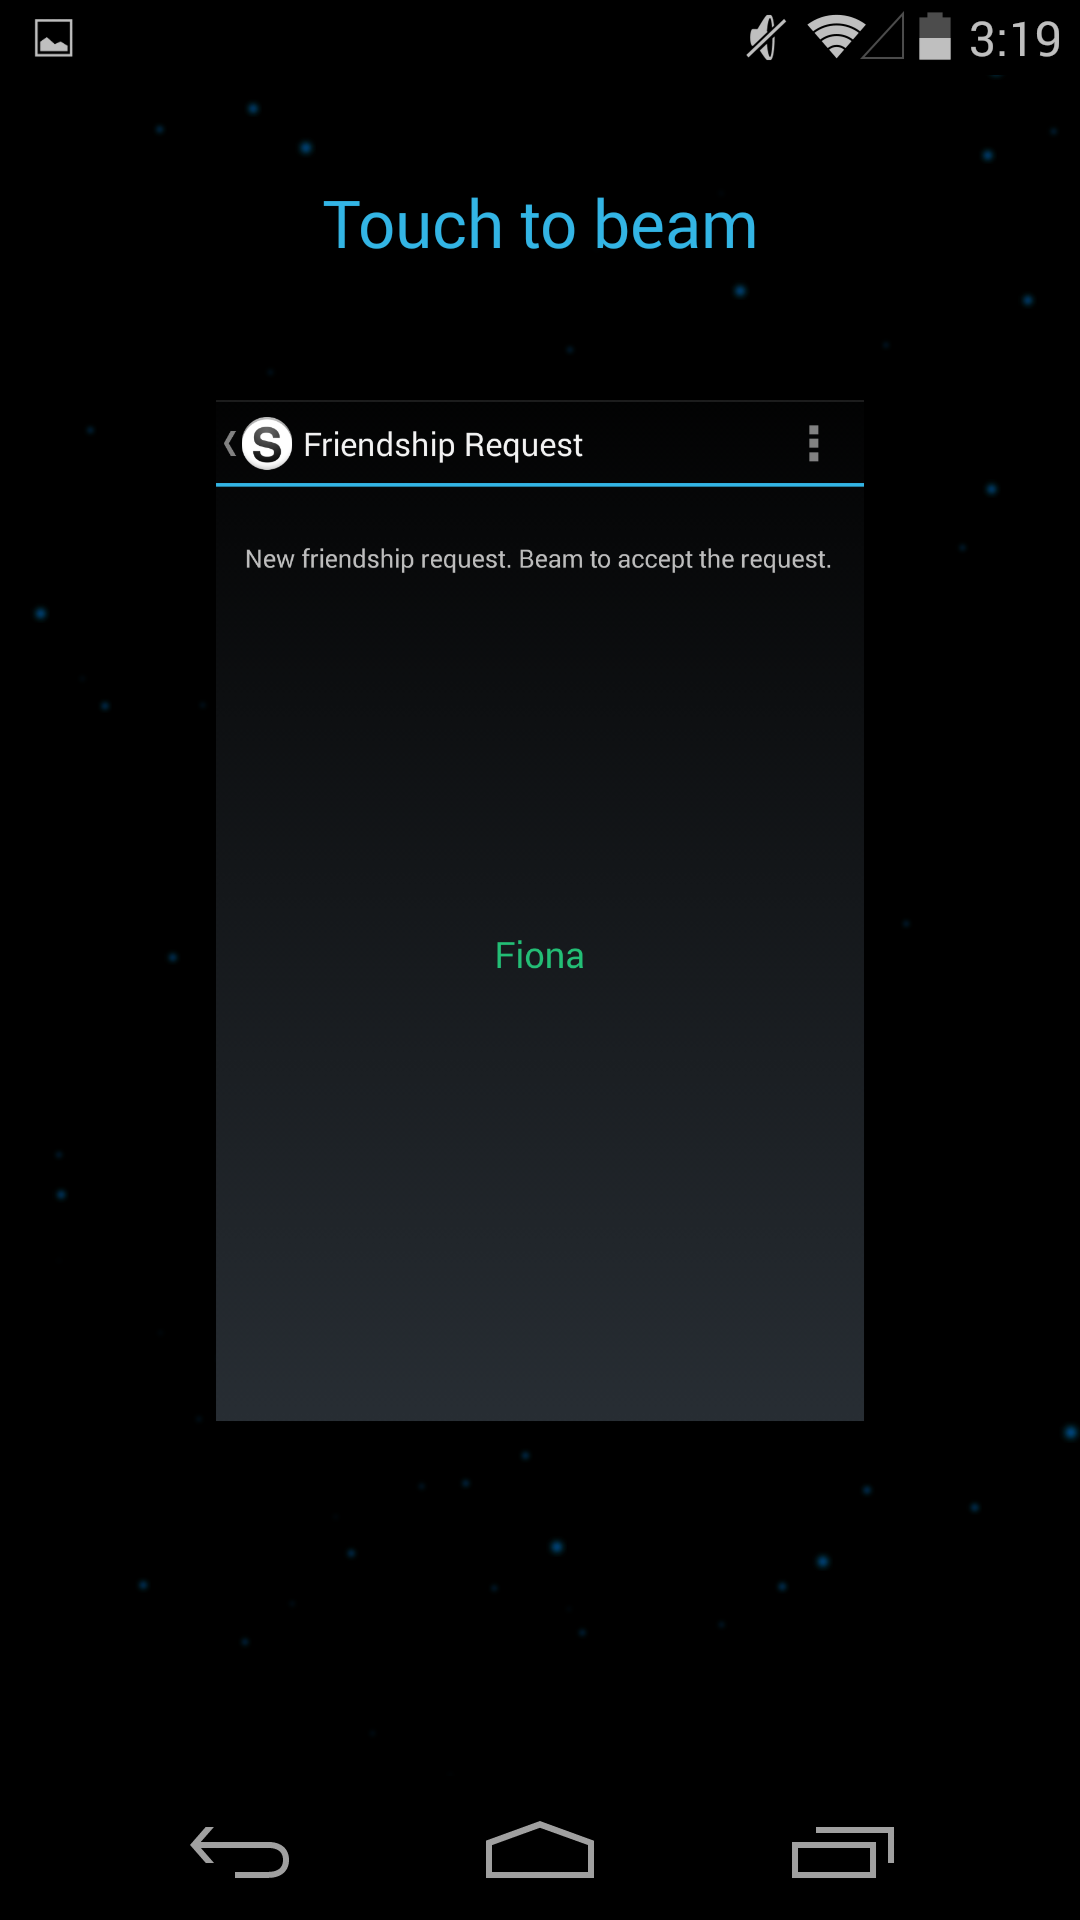
\includegraphics[height=4.5cm]{Figure_3}

	}
	
\end{figure}

Upon first opening the application, the user is prompted to choose a username for registration which then gets saved in the local database (d).

In the wall fragment the user can see an interface for adding new posts. There we have a button for adding pictures to a post. Pictures can be taken from the gallery or a new picture can be taken (e and f). A send button allows posting the content the user entered in the textView.

\begin{figure}[H]
	\centering
	\subfigure[]{
		\label{Figure a}
	    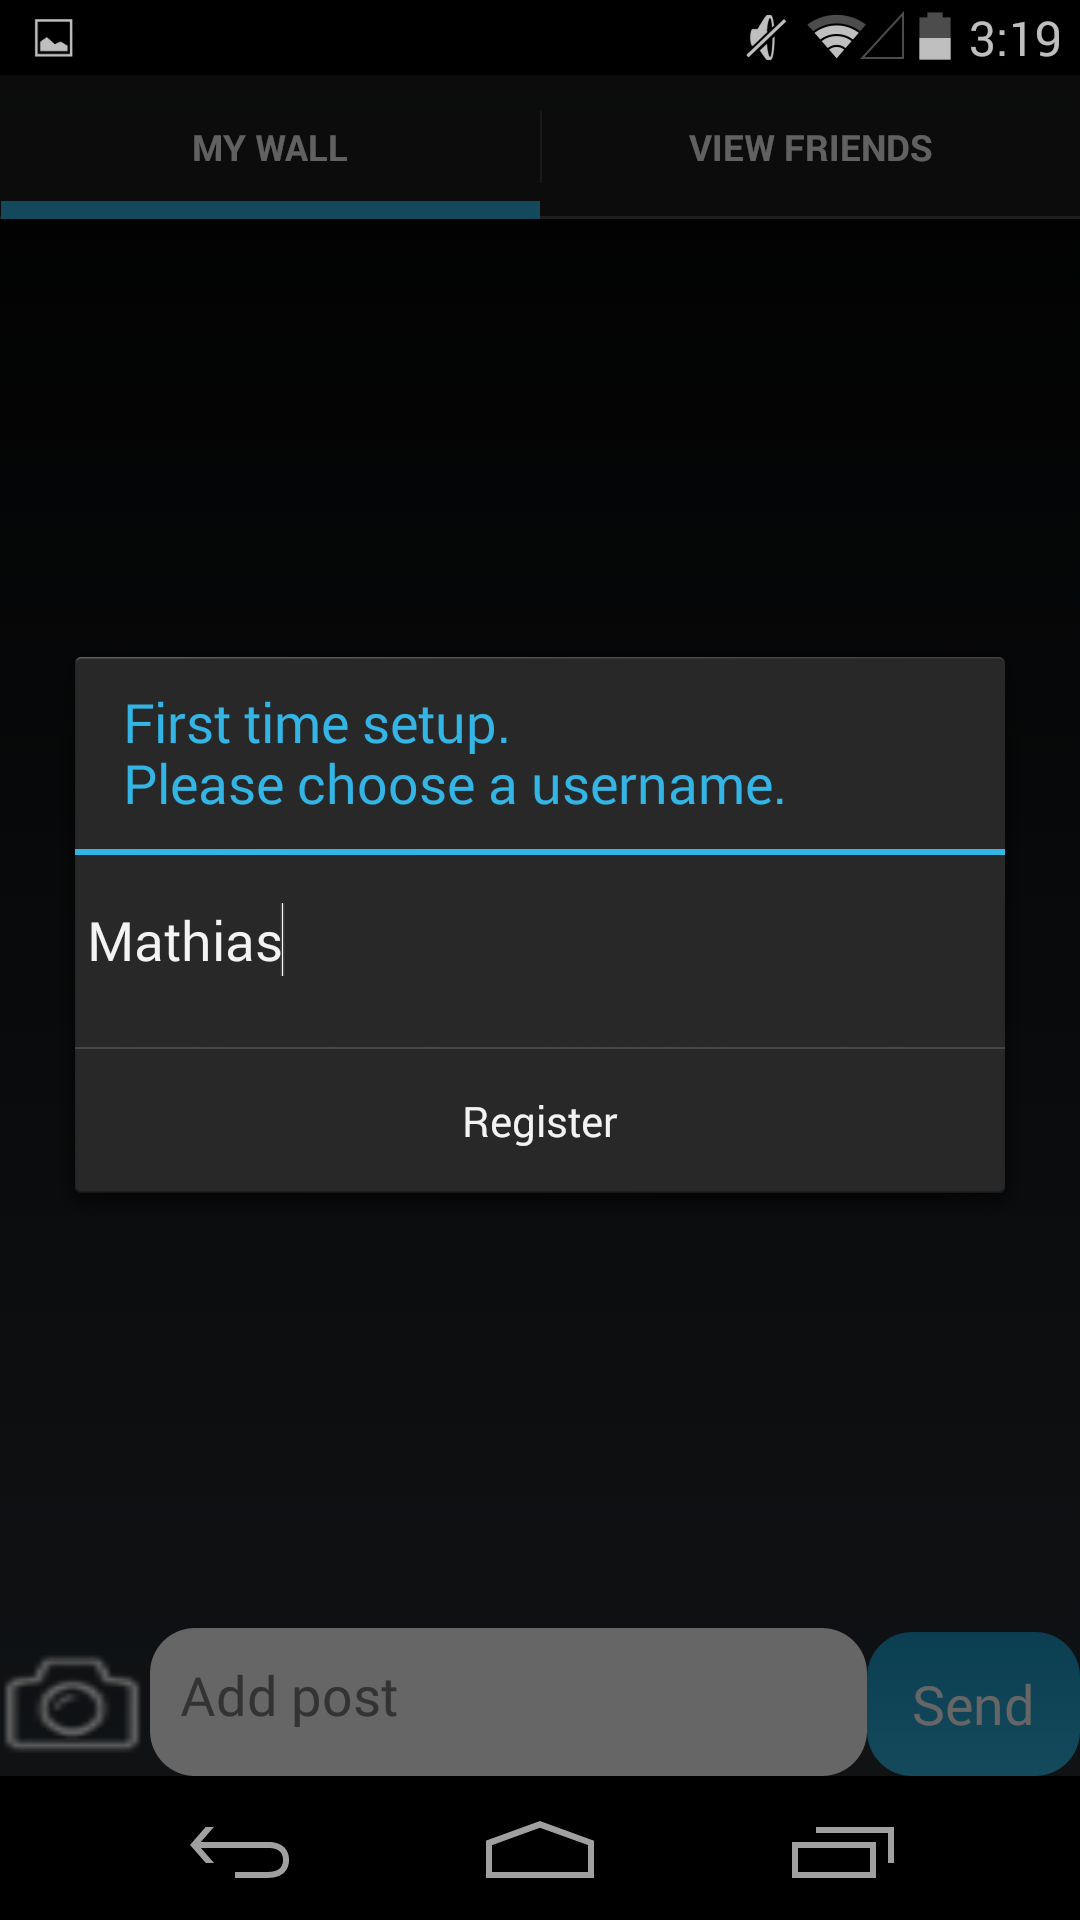
\includegraphics[height=4.5cm]{Figure_6}

	}
	\hfill
	\subfigure[]{
	    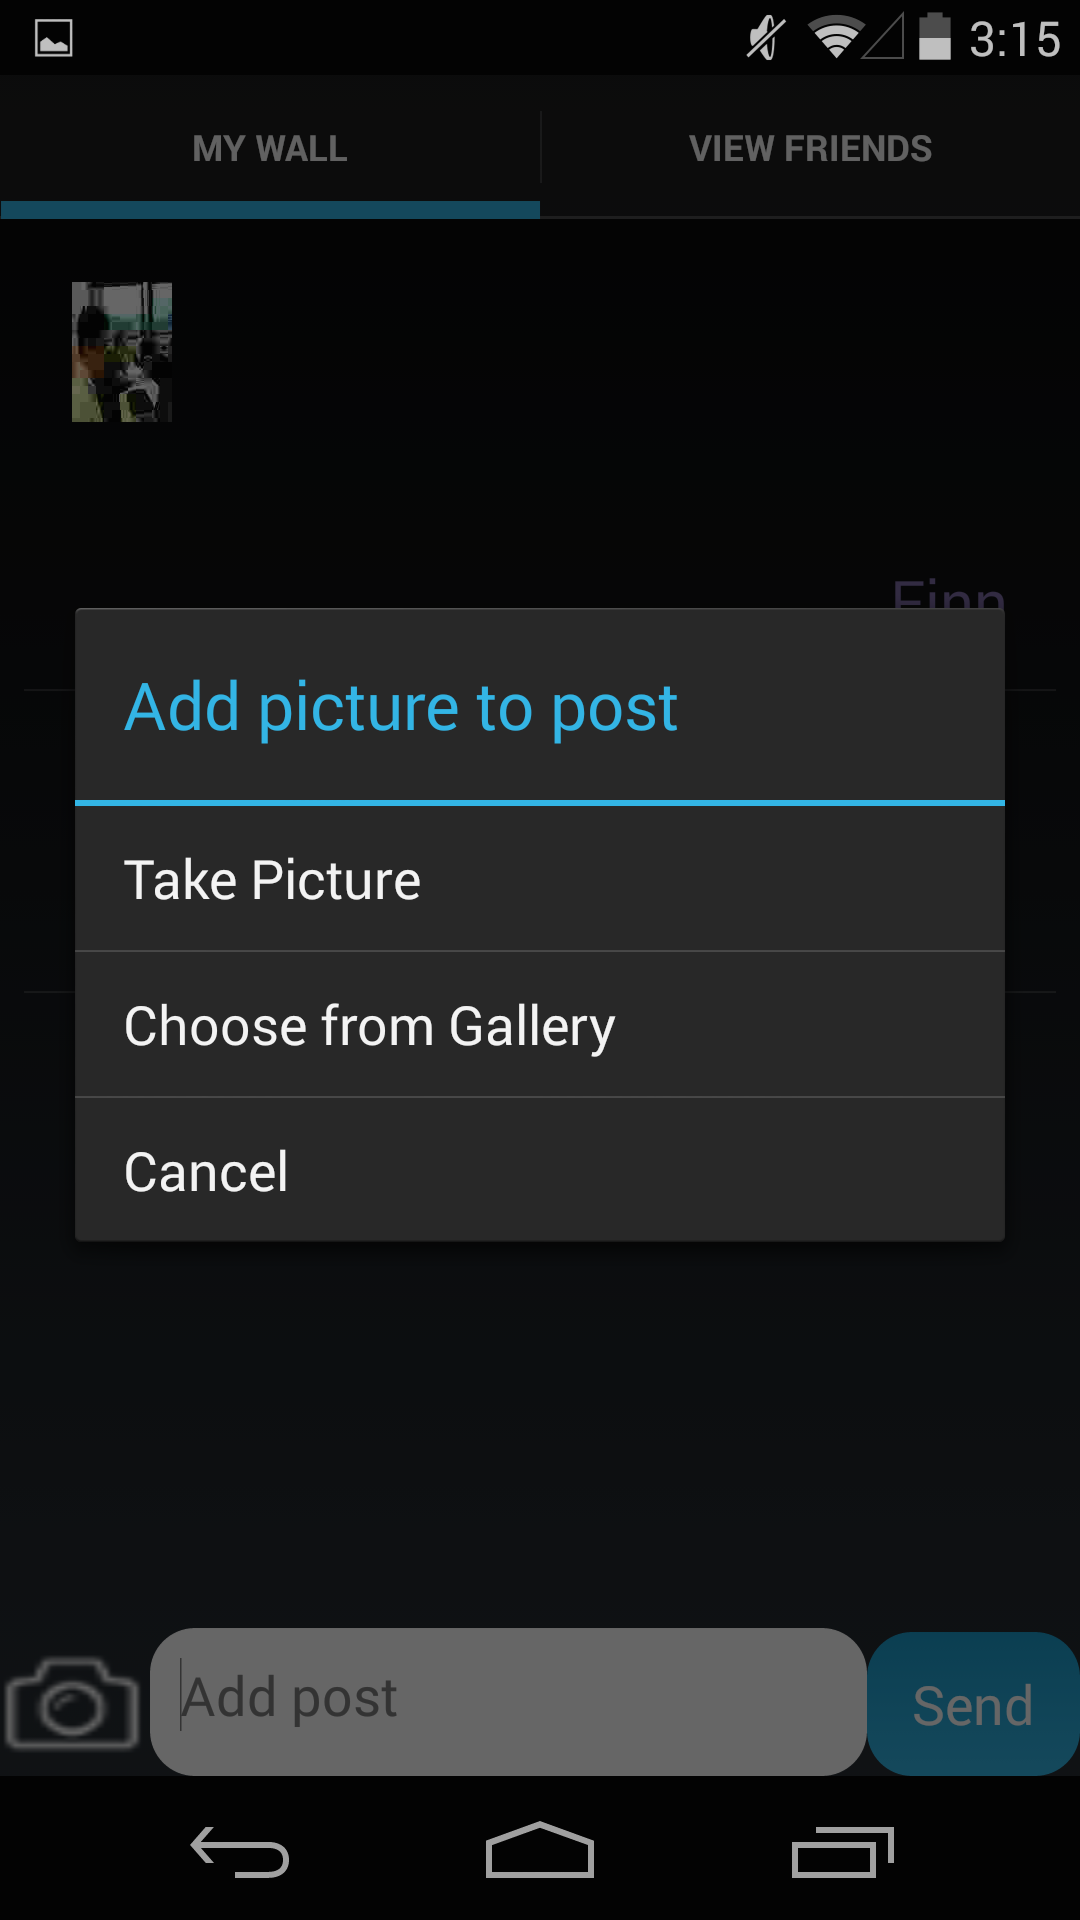
\includegraphics[height=4.5cm]{Figure_4}

	}
	\hfill
	\subfigure[]{
	    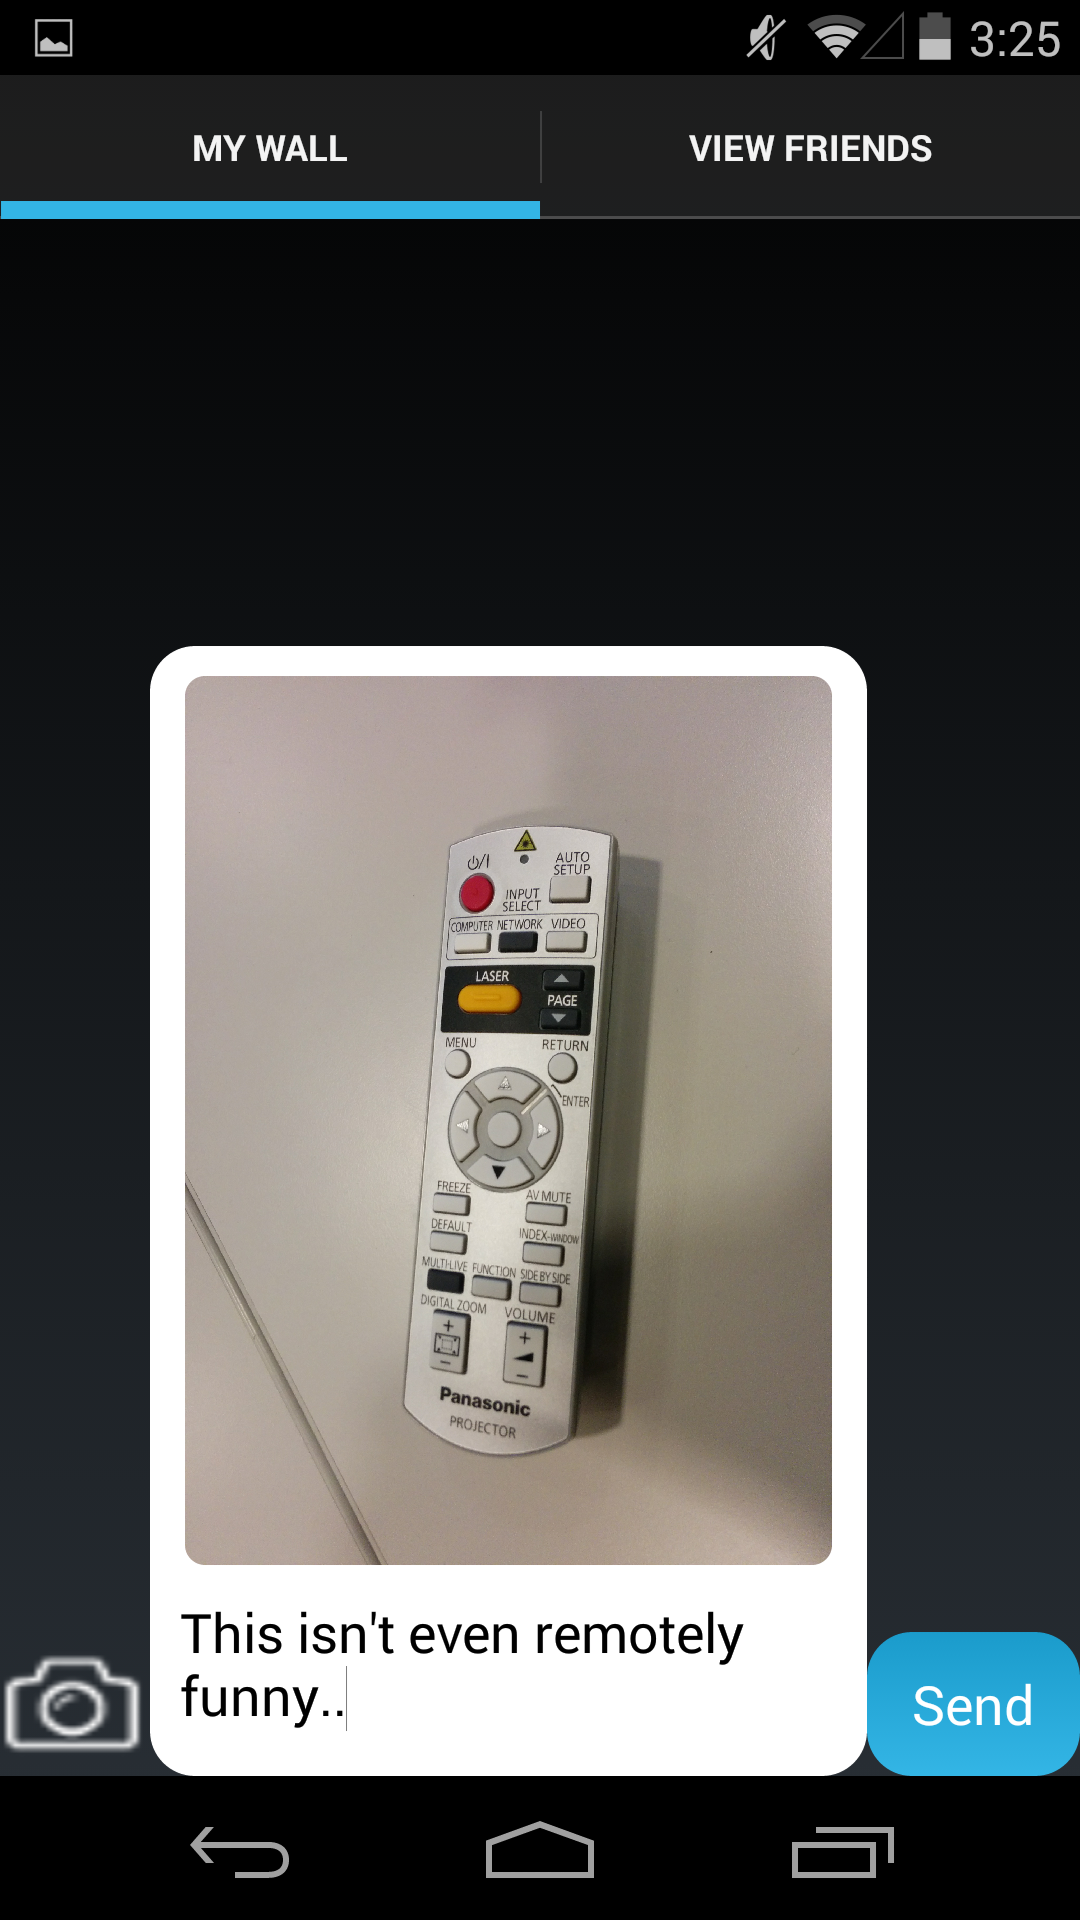
\includegraphics[height=4.5cm]{Figure_5}

	}
	
\end{figure}

\subsection{Protocol}

The main responsibility of the protocol lies in maintaining the eventual consistency of the system.

Each peer has a random 128-bit user id. This guarantees uniqueness of the ids with high probability without any coordination.
Each peer stores a post count and a virtual clock for each friend. The virtual clock is a lamport time stamp. We increment it when posting, and update it on receival of posts. Posts are ordered lexicographically with respect to the virtual clock and the user id of the author. This order is total for each wall.

Messages have a public header, which is sent in plain and used by the server for appropiate handling of the messages. The private part of a message consists of a JSON text portion and an optional image payload. (Figure 1)

\begin{figure}[H]

	\setcounter{figure}{0}
	\centering
    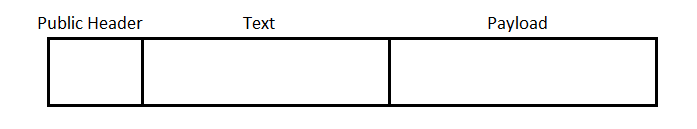
\includegraphics[width=\columnwidth]{Layout.png}
    \lfig{Layout}
    \vspace{-7mm} % use negative white space to fix too large gaps
    \label{Figure 1}
    \caption{layout of the whole message}
\end{figure}
\vspace{-3mm}
$\:$\newline
The layout of the public header is as follows:


\begin{figure}[H]

	\centering
    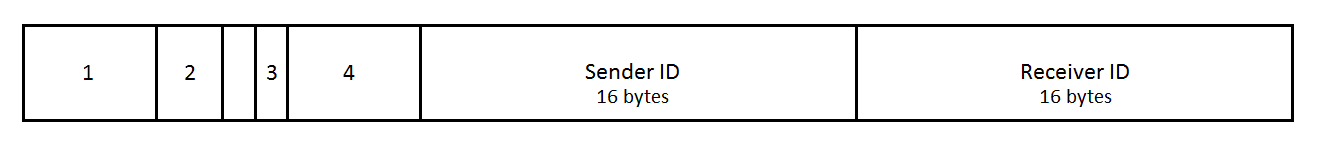
\includegraphics[width =\columnwidth]{PublicHeader.png}
    \lfig{PublicHeader}
    \vspace{-5mm} % use negative white space to fix too large gaps
\end{figure}

\vspace{-3mm}
$\:$\newline
1: length of the message (4 bytes) \newline
2: length of Text section (2 bytes)\newline
3: status byte (1 byte)\newline
4: virtual clock value (4 bytes)\newline
$\:$\newline
The protocol specifies the following events:\newline
\textbf{Request of data:} This happens when a peer wants to fetch updates of a certain wall.  
In case the target is the own wall it requests all buffered posts the server stored in its absence.
If it wants to access an other wall, there are two cases:\newline
Case 1 : Wall owner is online.
Responding to the data request, the target peer will send a message containing its wall's post count and virtual clock value. If the local post count is less than the reported post count, a request for all posts with value at least the reported virtual clock value is sent. The peer answeres this request by sending all such posts in increasing virtual clock value order. \newline
Case 2: Wall owner is offline.
In this case the server will send the peer all cached posts of the target peer's wall.\newline
\textbf{Making a post:}
As already mentioned, we increment the virtual clock of a wall when posting to it.\newline
In case the target is the own wall, the commit to the local database determines if the post is successful or not.
If the target is a friends wall, the instant the server receives the post message is decisive. The server has the responsibility of ensuring that such a post is delivered to the wall owner eventually. \newline
\textbf{Receiving a post:}
As previously outlined, whenever a post message is received the virtual clock value of the corresponding wall gets set to the maximum of the received value and the local value.  The wall's post count is incremented.

Under the assumption that messages are delivered reliably, and that the server does not crash the protocol works towards that the local views of the walls of the peeers are eventually consistent.  If someone posts on his or her own wall, then once the post has commited to the database, all friends will be able to retrieve that post by a data request at a later point. If a peer posts to some remote wall, by assumption the post will eventually be delivered to that peer. It is thus never the case that some peer thinks that its post was commited to the system, but it in fact never reaches the wall owner. This means that the local post count for an outdated wall is eventually below the post count of the post count of the wall owner, so eventually an update will be requested.

\subsection{Security}
The cryptography is peer-to-peer. The server acts as a relay for the client messages and is untrusted.

On first application start, every peer generates a broadcast key. A broadcast key is a pair $(k_1, k_2)$ where $k_1$ is used for encryption and $k_2$ for message authentication.

To establish a friendship, peers exchange their contact information and broadcast keys over Near-Field-Communication. Keys are exchanged in plain. This is reasonable under the assumption that the exchange occurs in a relatively private place.

To post a message on Bob's wall, Alice encrypts and authenticates the post under Bob's key and sends the post to the server for relaying to Bob and his friends. Since all friends of Bob share Bob's key, it is possible to post a message by encrypting it only once. Encryption is done by combining AES-128 [1] in CBC mode [2] and an HMAC [3] based on SHA256 [4] in an "Encrypt-then-Authenticate" fashion. More concretely the encryption function for message $m$ with public header $h$ is: \newline
$Enc_{(k_1, k_2)}(h|m) = h | MAC_{k_2}(h | Enc_{k_1}(m)) | Enc_{k_1}(m)$.
%footnotes for AES, CBC, HMAC, SHA256

% 1 AES: http://csrc.nist.gov/publications/fips/fips197/fips-197.pdf
% 2 CBC William F. Ehrsam, Carl H. W. Meyer, John L. Smith, Walter L. Tuchman, "Message verification and transmission error detection by block chaining", US Patent 4074066, 1976
% 3 HMAC http://tools.ietf.org/html/rfc2104
% 4 SHA https://www.federalregister.gov/articles/2012/03/06/2012-5400/announcing-approval-of-federal-information-processing-standard-fips-publication-180-4-secure-hash

Assuming that no friends are compromised, this gives us authenticity and secrecy for the transmission of posts. A compromised peer exposes the communication of all of his or her friends. However, it is very expensive to eavesdrop or manipulate communication on a large scale, as there is no central storage or transmission of key material.

\subsection{Database}
%Structure
In order to store persistently the user's data on his or her device it tourned out that the most suitable approach between the ones offered by the Android operating system [5], was to use a SQLite database [6]. This decision was mainly based on the two following application requirements:\newline
1) the user data needs to be structured;\newline
2) it shouldn't be possible to access the data from outside the application;\newline
The structure of the database is simple and consists of only two tables: one storing the users' data and the other storing the posts.

The user table (Figure 1) stores id, username and other information needed by different layers, e.g. the number of messages on the user's wall for the protocol layer and the keys for the secutity layer. The primary key is the id, since it's unique with high probability among all users.

\begin{figure}[H]
	
	
	\centering
    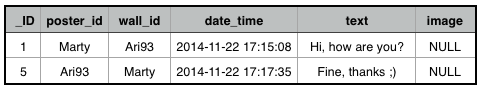
\includegraphics[width=\columnwidth]{users_table_example.png}
    \lfig{users_table_example}
    \vspace{-5mm} % use negative white space to fix too large gaps
	\caption{user table with example data ("..."$\:$ means that the data is too long to fit)}
\end{figure}

The post table (Figure 2) stores the single posts that are part of the user's wall or one of his/hers friend's wall. 
A post contains an id, the id of who posted it, the id of the user on whose wall it was posted, date and time when it was received, text and/or image content.Id, poster$\_$id and wall$\_$id form the primary key, while both poster$\_$id and wall$\_$id are foreign key references to the users table.

\begin{figure}[H]
	\centering
    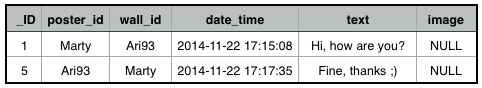
\includegraphics[width=\columnwidth]{post_table_example.png}
    \lfig{post_table_example}
    \vspace{-5mm} % use negative white space to fix too large gaps
	\caption{post table with example data}
\end{figure}

%Implementation

An interface provides access to the functionalities of the database for the other layers, which don't have another way to access the data. This allows a better control over the state of the database, in particular for assuring consistency to the whole system, and made easier throughout the implementation process, because the structure and the methods evolved over time.
Extending the SQLiteOpenHelper class [7] helped to make database creation and version control easier to manage.
All core methods are implemented using the functions already provided by the SQLiteDatabase class [8], in particular insert(), update(), delete() and query(). This methods are divided into three categories:
- user, to manage data about the owner of the device;
- friend, to manage data about all his or her friends;
- post, to manage data about all posts saved in the device.



\subsection{Server and Networking}

\vspace{-1mm}
$\:$\newline
\textbf{Hardware and Setup}\newline
\indent The server in our project is only responsible for forwarding, buffering and caching the messages. It doesn't store the user data in a permanent way and also cannot read the user messages, since the data is encrypted. 
Because of these circumstances we decided on having a small, lightweight server. Therefore we used a Raspberry Pi Modell B [9]. The R-Pi runs an ARM 700 MHz processor and 512 MB of RAM. It is connected with an Ethernet cable to the network.
The R-Pi is running Raspbian, a linux distribution, adapted for Raspberry Pi devices. The whole installation is headless and accessed through SSH. This setup is very energy efficient. 
Since we do not have access to a static Public IP, we have a client in the network, that updates a DNS entry [10] every minute and guarantees, that our server is always reachable over the same address. 

\vspace{-2mm}
$\:$\newline
\textbf{Software}\newline
\indent Because of the limited resources the hardware is offering the server application needs to be very lightweight. To avoid too much thread-switching overhead, to efficiently use the resources and offer good scalability, we decided on a Non-blocking I/O (NIO) [11][12] approach to design the server application. The core-application consists of two threads running in parallel. The server thread, which implements the NIO server and a worker thread which processes the incoming data and decides what to do with the messages. Based on the public header the worker thread handles the message accordingly.
%Two data structures are responsible to process the messages in a meaningful way. The first is a HashMap which stores the connected users and the corresponding sockets. If a user is not connected, then the posts get buffered in a user specific PriorityQueue. The time a user connects again he or she can request all posts on his or her wall missed whilst offline.
Alongside the core-application, a monitor thread is running. The task of the monitor thread is to periodically check the connectivity and memory usage of the application. In case of failure and/or too less memory available, the monitor thread can command the server to drop the oldest messages in the cache or to restart the server thread. 

\vspace{-2mm}
$\:$\newline
\textbf{Transport Protocol}\newline
\indent Communication is performed over TCP. This allows us to rely on the correct ordering and reliable transmission of messages.

\section{Testing}

We have implemented unit tests for the non-interactive components. This includes a dummy client testing the server and correctness tests for security, database and client protocol implementation.

Integration tests were performed interactively.

\section{Outlook}

The reliance on a message relaying server could be further reduced by enabling peers to directly communicate. The main issue in implementing this is NAT-traversal, though solutions to achieve this exist.

The security of the key exchange mechanism could be improved by first exchanging some public keys, and then exchanging the broadcast keys encrypted under those public keys.

One issue is that current monetization models seem hard to apply to our approach, as no information about the content users are sharing is available. To provide userful advertisement, the pseudo-anonymous network information available to the server might prove to be sufficient. 

\section{Conclusion}

Mobile devices are powerful enough to implement a mostly peer-to-peer social network. Our architecture might provide reduced infrastructure costs compared to centralized systems, as little or no permanent storage is required. Availability is acceptable: Users can always access content they have seen before, and eventually they will receive all updates. 
The system should scale well, as the server component could be very easily replicated without the need for complex synchronisation mechanisms.

\section{References}
\vspace{-3mm}
$\:$\newline
[1] AES: http://csrc.nist.gov/publications/fips/fips197/fips-197.pdf\newline
[2] CBC William F. Ehrsam, Carl H. W. Meyer, John L. Smith, Walter L. Tuchman,
"Message verification and transmission error detection by block chaining", US Patent 4074066, 1976\newline
[3] HMAC http://tools.ietf.org/html/rfc2104\newline
[4] SHA https://www.federalregister.gov/articles/\newline2012/03/06/2012-5400/ announcing-approval-of-federal-information-processing-standard-fips-publication-180-4-secure-hash\newline
[5] http://developer.android.com/guide/topics/data/\newline data-storage.html\newline
[6] http://developer.android.com/training/basics/data-storage/\newline databases.html\newline
[7] http://developer.android.com/reference/android/database/\newline sqlite/SQLiteOpenHelper.html\newline
[8] http://developer.android.com/reference/android/database/\newline sqlite/SQLiteDatabase.html\newline
[9] http://www.raspberrypi.org/\newline
[10] freedns.afraid.org\newline
[11] http://en.wikipedia.org/wiki/Non-blocking$\_$I/O$\_$$\%$28Java$\%$29\newline
[12] http://docs.oracle.com/javase/7/docs/api/java/nio/channels/\newline package-summary.html\newline



% The following two commands are all you need in the
% initial runs of your .tex file to
% produce the bibliography for the citations in your paper.
\bibliographystyle{abbrv}
\bibliography{report}  % sigproc.bib is the name of the Bibliography in this case
% You must have a proper ".bib" file

%\balancecolumns % GM June 2007

\end{document}
